\documentclass{article}
\usepackage[a4paper,margin=1in,landscape]{geometry}

\usepackage{booktabs}

\usepackage{graphicx}
\usepackage{booktabs}
\usepackage{amsmath}
\usepackage{longtable}
\usepackage{array}
\usepackage{pgf-pie}
\usepackage{pgfplots}

\begin{document}



\section*{BUILDING INFORMATION}
\begin{longtable}{| l | l |}
\hline
\textbf{Category:} & Residential \\
\hline
\textbf{Status:} & in planning \\
\hline
\textbf{Building type:} & New construction \\
\hline
\textbf{Year of construction:} & 0 \\
\hline
\textbf{Units:} & 1 \\
\hline
\textbf{Number of occupants:} & 3 (Design) \\
\hline
\textbf{Occupant density:} & 51 \, $m^2$/Person \\
\hline
\end{longtable}

\section*{Boundary conditions}
\begin{longtable}{| l | l |}
\hline
\textbf{Climate:} & User defined \\
\hline
\textbf{Internal heat gains:} & 2.3 \, $W/m^2$ \\
\hline
\textbf{Interior temperature:} & 20 \, °C \\
\hline
\textbf{Overheat temperature:} & 25 \, °C \\
\hline
\end{longtable}

\section*{Building geometry}
\begin{longtable}{| l | l |}
\hline
\textbf{Enclosed volume:} & 590.4 \, $m^3$ \\
\hline
\textbf{Net-volume:} & 463.4 \, $m^3$ \\
\hline
\textbf{Total area envelope:} & 439.2 \, $m^2$ \\
\hline
\textbf{Area/Volume Ratio:} & 0.7 \, 1/m \\
\hline
\textbf{Floor area:} & 153 \, $m^2$ \\
\hline
\textbf{Envelope area/ICFA:} & 2.871 \\
\hline
\end{longtable}

\section*{PASSIVEHOUSE REQUIREMENTS}
\textbf{Certificate criteria:} Phius CORE 2021

\subsection*{Heating demand}
\begin{longtable}{| l | l |}
\hline
\textbf{Specific:} & 5.07 \, kWh/m²a \\
\hline
\textbf{Target:} & 15 \, kWh/m²a \\
\hline
\textbf{Total:} & 776.17 \, kWh/a \\
\hline
\end{longtable}

\subsection*{Cooling demand}
\begin{longtable}{| l | l |}
\hline
\textbf{Sensible:} & 11.39 \, kWh/m²a \\
\hline
\textbf{Latent:} & 3.29 \, kWh/m²a \\
\hline
\textbf{Specific:} & 14.69 \, kWh/m²a \\
\hline
\textbf{Target:} & 15 \, kWh/m²a \\
\hline
\textbf{Total:} & 2,246.53 \, kWh/a \\
\hline
\end{longtable}

\subsection*{Heating load}
\begin{longtable}{| l | l |}
\hline
\textbf{W/m²:} & 8.66 \, W/m² \\
\hline
\textbf{Target:} & 10 \, W/m² \\
\hline
\textbf{Total:} & 1,325.03 \, W \\
\hline
\end{longtable}

\subsection*{Cooling load}
\begin{longtable}{| l | l |}
\hline
\textbf{Specific:} & 9.71 \, W/m² \\
\hline
\textbf{Total:} & W/m² \\
\hline
\end{longtable}


\section*{Annual Heat Demand}

\begin{tabular}{@{}ll@{}}


\toprule
\textbf{Item} &
\textbf{Value (kWh/a)} \\
\midrule
Transmission losses & 5,455
\\
Ventilation losses & 1,216 \\
Total heat losses & 6,671 \\
Solar heat gains & 5,455 \\
Internal heat gains & 1,270 \\
Total heat gains & 6,725 \\
Utilization factor & 87.7\% \\
Useful heat gains & 5,895 \\
\midrule
Annual heat demand & 776 \\
Specific annual heat demand & 5.1 \\
\bottomrule
\end{tabular}

\vspace{1cm}
\section*{Annual Cooling Demand}
\begin{tabular}{@{}ll@{}}
\toprule
\textbf{Item} & \textbf{Value (kWh/a)} \\ \midrule
Solar heat gains & 2,242 \\
Internal heat gains & 2,482 \\
Total heat gains & 4,724 \\
Transmission losses & 2,928 \\
Ventilation losses & 509 \\
Total heat losses & 3,437 \\
Utilization factor & 86.7\% \\
Useful heat losses & 2,981 \\
\midrule
Cooling demand - sensible & 1,743 \\
Cooling demand - latent & 503 \\
Annual cooling demand & 2,247 \\
Specific annual cooling demand & 14.7 \\
\bottomrule
\end{tabular}

\section*{Source Energy}
\begin{itemize}
    \item Total: $11,649.6$ kWh/a
    \item Specific: $3,883$ kWh/Person a
    \item Target: $4,850$ kWh/Person a
    \item Specific: $76.15$ kWh/m$^2$a
\end{itemize}

\section*{Site Energy}
\begin{itemize}
    \item Total: $6,472$ kWh/a
    \item Specific: $42.31$ kWh/m$^2$a
\end{itemize}

\section*{Air Tightness}
\begin{itemize}
    \item ACH$_{50}$: $0.85$ 1/h
    \item CFM$_{50}$ per envelope area: $0.9$ m$^3$/m$^2$h
    \item Target: $1.04$ 1/h
    \item Target CFM$_{50}$: $1.1$ m$^3$/m$^2$h
\end{itemize}

\section*{Passive House Recommendations}
\begin{itemize}
    \item Sensible Recovery Efficiency: $75.7\%$
    \item Frequency of Overheating: $33.4\%$ \\
    \textit{Cooling system is required.}
\end{itemize}
\textit{Frequency of overheating only applies if there is not a [properly sized] cooling system installed.}


\section*{Building Elements}

\subsection*{Windows}

\begin{tabular}{|l|l|}
    \hline
    Average SHGC & 0.47 \\
    \hline
    Average Solar Reduction Factor (Heating) & 0.51 \\
    \hline
    Average Solar Reduction Factor (Cooling) & 0.1 \\
    \hline
    Average U-value & 0.799 W/m²K \\
    \hline
    Total Glazing Area & 53.8 m² \\
    \hline
    Total Window Area & 67.9 m² \\
    \hline
\end{tabular}

\vspace{1cm}

\subsection*{HVAC}

\begin{tabular}{|l|l|}
    \hline
    Total Heating Demand & 776 kWh/a \\
    \hline
    Total Cooling Demand & 2,247 kWh/a \\
    \hline
    Total DHW Energy Demand & 2,824 kWh/a \\
    \hline
    Solar DHW Contribution & 0 kWh/a \\
    \hline
    Auxiliary Electricity & 231 kWh/a \\
    \hline
\end{tabular}

\vspace{1cm}

\subsection*{Electricity}

\begin{tabular}{|l|l|}
    \hline
    Direct Heating / DHW & 2,288 kWh/a \\
    \hline
    Cooling & 478 kWh/a \\
    \hline
    HVAC Auxiliary Energy & 231 kWh/a \\
    \hline
    Appliances & 3,476 kWh/a \\
    \hline
    Renewable Generation & 0 kWh/a \\
    \hline
    Total Electricity Demand & 6,472 kWh/a \\
    \hline
\end{tabular}

\vspace{1cm}

\section*{Heat Flow - Heating Period}

\subsection*{Heat Gains}

\begin{tabular}{|l|l|}
    \hline
    Solar & 4,781 kWh/a \\
    \hline
    Inner Sources & 1,114 kWh/a \\
    \hline
    Credit of Thermal Bridges & 0 kWh/a \\
    \hline
    Mechanical Heating & 776 kWh/a \\
    \hline
\end{tabular}

\vspace{1cm}

\subsection*{Heat Losses}

\begin{tabular}{|l|l|}
    \hline
    Opaque Building Envelope & 2,443 kWh/a \\
    \hline
    Windows \& Doors & 2,957 kWh/a \\
    \hline
    Natural Ventilation & 712 kWh/a \\
    \hline
    Mechanical Ventilation & 504 kWh/a \\
    \hline
\end{tabular}

\vspace{1cm}

\subsection*{Pie Charts}

\begin{minipage}{0.45\textwidth}
    \centering
    \textbf{Heat Gains Distribution}
    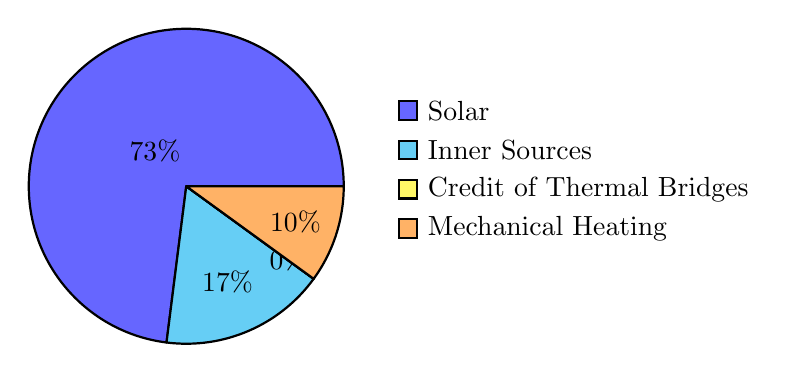
\begin{tikzpicture}
        \pie[text=legend, radius=2]{73/Solar, 17/Inner Sources, 0/Credit of Thermal Bridges, 10/Mechanical Heating}
    \end{tikzpicture}
\end{minipage}
\hspace{1cm}
\begin{minipage}{0.45\textwidth}
    \centering
    \textbf{Heat Losses Distribution}
    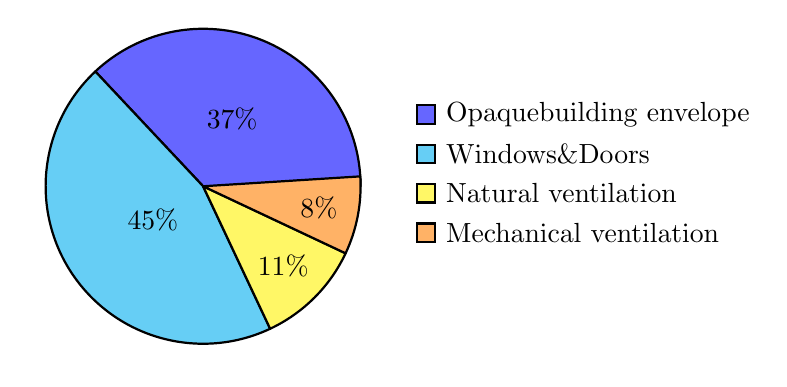
\begin{tikzpicture}
        \pie[text=legend, radius=2]{37/Opaquebuilding envelope, 45/Windows\&Doors, 11/Natural ventilation, 8/Mechanical ventilation}
    \end{tikzpicture}
\end{minipage}


\section*{CLIMATE}

\begin{itemize}
    \item Latitude: 42.6 °
    \item Longitude: 27.5 °
    \item Elevation of weather station: 41.1 m
    \item Elevation of building site: 41.1 m
    \item Heat capacity air: 0.33 Wh/m\textsuperscript{2}K
    \item Daily temperature swing summer: 8 K
    \item Average wind speed: 4.1 m/s
\end{itemize}

\subsection*{Ground}

\begin{itemize}
    \item Average ground surface temperature: 14.1 °C
    \item Amplitude ground surface temperature: 10.8 °C
    \item Ground thermal conductivity: 2 W/mK
    \item Ground heat capacity: 2 MJ/m\textsuperscript{2}K
    \item Depth below grade of groundwater: 3 m
    \item Flow rate groundwater: 0.1 m/d
\end{itemize}

\subsection*{Calculation parameters}

\begin{itemize}
    \item Length of heating period: 151 days/a
    \item Heating degree hours: 59.2 kKh/a
    \item Phase shift months: 1.3 months
    \item Time constant heating demand: 223.3 h
    \item Time constant cooling demand: 0 h
    \item Time constant cooling demand with night ventilation: 0 h
\end{itemize}

\begin{table}[h!]
    \centering
    \begin{tabular}{@{}lcccccc@{}}
        \toprule
        Climate for & Heating load 1 & Heating load 2 & Cooling \\ \midrule
        Temperature [°C] & -11.1 & -11.1 & 31 \\
        Solar radiation North [W/m²] & 49 & 49 & 78 \\
        Solar radiation East [W/m²] & 93 & 93 & 108 \\
        Solar radiation South [W/m²] & 206 & 206 & 100 \\
        Solar radiation West [W/m²] & 109 & 109 & 112 \\
        Solar radiation Global [W/m²] & 124 & 124 & 209 \\ \bottomrule
    \end{tabular}
    \caption{Relevant boundary conditions for heating load calculation: Heating load 1}
\end{table}


\begin{table}[h!]
    \centering
    \caption{Annual Heat Demand}
    \begin{tabular}{@{}ll@{}}
        \toprule
        \textbf{Description}         & \textbf{kWh/a} \\ \midrule
        Transmission losses          & 5,455          \\
        Ventilation losses           & 1,216          \\
        Total heat losses            & 6,671          \\
        Solar heat gains             & 5,455          \\
        Internal heat gains          & 1,270          \\
        Total heat gains             & 6,725          \\
        Utilization factor           & 87.7\%         \\
        Useful heat gains            & 5,895          \\ \midrule
        Annual heat demand           & 776            \\
        Specific annual heat demand   & 5.1 kWh/m²     \\ \bottomrule
    \end{tabular}
\end{table}

\begin{table}[h!]
    \centering
    \caption{Annual Cooling Demand}
    \begin{tabular}{@{}ll@{}}
        \toprule
        \textbf{Description}         & \textbf{kWh/a} \\ \midrule
        Solar heat gains             & 2,242          \\
        Internal heat gains          & 2,482          \\
        Total heat gains             & 4,724          \\
        Transmission losses          & 2,928          \\
        Ventilation losses           & 509            \\
        Total heat losses            & 3,437          \\
        Utilization factor           & 86.7\%         \\
        Useful heat losses           & 2,981          \\ \midrule
        Cooling demand - sensible     & 1,743          \\
        Cooling demand - latent       & 503            \\
        Annual cooling demand         & 2,247          \\
        Specific annual cooling demand & 14.7 kWh/m²    \\ \bottomrule
    \end{tabular}
\end{table}


\begin{center}
    \textbf{SPECIFIC HEAT/COOLING DEMAND MONTHLY}
\end{center}

\begin{table}[h]
    \centering
    \caption{Monthly Heating and Cooling Demand}
    \begin{tabular}{@{}llcc@{}}
        \toprule
        Month      & Heating [kWh/m²] & Cooling [kWh/m²] \\
        \midrule
        January    & 1.9              & 0                \\
        February   & 0.9              & 0                \\
        March      & 0                & 0                \\
        April      & 0                & 0                \\
        May        & 0                & 0.1              \\
        June       & 0                & 2.8              \\
        July       & 4.8              & 0                \\
        August     & 5.1              & 0                \\
        September   & 1.8              & 0                \\
        October    & 0                & 0                \\
        November   & 0                & 0                \\
        December   & 2.2              & 0                \\
        \bottomrule
    \end{tabular}
    \label{tab:heating_cooling}
\end{table}


\section*{Heating Load}

\begin{table}[h!]
    \centering
    \caption{Heating Load Data}
    \begin{tabular}{@{}lll@{}}
        \toprule
        \textbf{Parameter} & \textbf{First Climate} & \textbf{Second Climate} \\ \midrule
        Transmission heat losses: & 3,004.8 W & 3,004.8 W \\
        Ventilation heat losses: & 1,301.5 W & 1,301.5 W \\
        Total heat loss: & 4,306.3 W & 4,306.3 W \\
        Solar heat gain: & 2,736.5 W & 2,736.5 W \\
        Internal heat gain: & 244.8 W & 244.8 W \\
        Total heat gains heating: & 2,981.3 W & 2,981.3 W \\ \midrule
        Heating load: & 1,325 W & 1,325 W \\ \midrule
        Relevant heating load: & 1,325 W &  \\
        Specific heating load: & 8.7 W/m² &  \\
        \bottomrule
    \end{tabular}
\end{table}

\section*{Cooling Load}

\begin{table}[h!]
    \centering
    \caption{Cooling Load Data}
    \begin{tabular}{@{}lll@{}}
        \toprule
        \textbf{Parameter} & \textbf{Value} \\ \midrule
        Solar heat gain: & 403.1 W \\
        Internal heat gain: & 562.1 W \\
        Total heat gains cooling: & 965.2 W \\
        Transmission heat losses: & -386.7 W \\
        Ventilation heat losses: & -133.7 W \\
        Total heat loss: & -520.4 W \\ \midrule
        Cooling load - sensible: & 1,485.6 W \\
        Cooling load - latent: & 0 W \\ \midrule
        Relevant cooling load: & 1,485.6 W \\
        Specific maximum cooling load: & 9.7 W/m² \\
        \bottomrule
    \end{tabular}
\end{table}

\section*{Energy Balance}

\begin{figure}[h!]
    \centering
    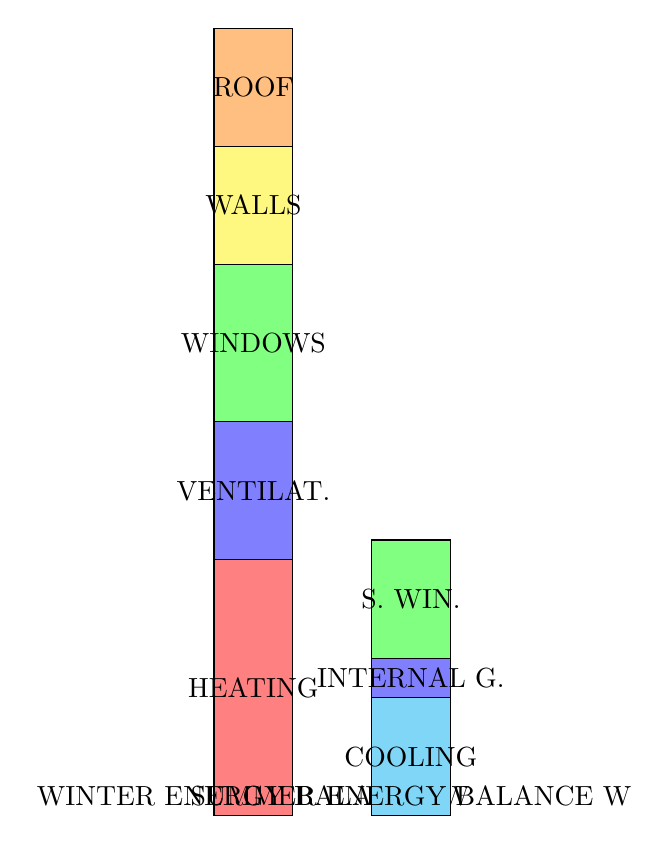
\begin{tikzpicture}
        % Winter Energy Balance
        \draw[fill=red!50] (0,0) rectangle (1,3.25) node[pos=0.5] {HEATING};
        \draw[fill=blue!50] (0,3.25) rectangle (1,5) node[pos=0.5] {VENTILAT.};
        \draw[fill=green!50] (0,5) rectangle (1,7) node[pos=0.5] {WINDOWS};
        \draw[fill=yellow!50] (0,7) rectangle (1,8.5) node[pos=0.5] {WALLS};
        \draw[fill=orange!50] (0,8.5) rectangle (1,10) node[pos=0.5] {ROOF};

        \node[anchor=south] at (0.5,0) {WINTER ENERGY BALANCE W};

        % Summer Energy Balance
        \draw[fill=cyan!50] (2,0) rectangle (3,1.5) node[pos=0.5] {COOLING};
        \draw[fill=blue!50] (2,1.5) rectangle (3,2) node[pos=0.5] {INTERNAL G.};
        \draw[fill=green!50] (2,2) rectangle (3,3.5) node[pos=0.5] {S. WIN.};

        \node[anchor=south] at (2.5,0) {SUMMER ENERGY BALANCE W};
    \end{tikzpicture}
\end{figure}



\section*{AREAS}
\begin{table}[h!]
    \centering
    \caption{Transmission heat losses - areas}
    \begin{tabular}{@{}lcccccccc@{}}
        \toprule
        Name & Area $[m^2]$ & Average U-value $[W/m^2K]$ & Absorption coefficient & Emission coefficient & Reduction factor shading [\%] & Transmission losses heating $[kWh/a]$ & Transmission losses cooling $[kWh/a]$ \\
        \midrule
        VC.1: FLOOR [ground floor]: Horizontal (98.4 m², width 12 m) & 98.4 & 0.271 & 0.4 & 0 & 0 & 498.3 & 499.8 \\
        VC.2: ROOF\_CEILING [roof]: Horizontal (98.4 m², width 12 m) & 96.4 & 0.115 & 0.4 & 0 & 0 & 624.5 & 267.7 \\
        VC.3: WALL [ext wall]: SW (A225°, 17.96 m², width 12 m) & 17.96 & 0.139 & 0.4 & 0 & 0 & 135.9 & 64.4 \\
        VC.3: WALL [ext wall]: SE (A135°, 16.48 m², width 8.2 m) & 16.48 & 0.139 & 0.4 & 0 & 0 & 124.7 & 59.4 \\
        VC.3: WALL [ext wall]: NE (A45°, 33.48 m², width 12 m) & 33.48 & 0.139 & 0.4 & 0 & 0 & 253.3 & 120.7 \\
        VC.3: WALL [ext wall]: NW (A315°, 19.76 m², width 8.2 m) & 19.76 & 0.139 & 0.4 & 0 & 0 & 64.9 & 41.1 \\
        VC.3: WALL [ext wall]: SW (A225°, 17.96 m², width 12 m) & 17.96 & 0.139 & 0.4 & 0 & 0 & 135.9 & 64.4 \\
        VC.3: WALL [ext wall]: SE (A135°, 16.48 m², width 8.2 m) & 16.48 & 0.139 & 0.4 & 0 & 0 & 124.7 & 59.4 \\
        VC.3: WALL [ext wall]: NE (A45°, 33.48 m², width 12 m) & 33.48 & 0.139 & 0.4 & 0 & 0 & 253.3 & 120.7 \\
        VC.3: WALL [ext wall]: NW (A315°, 18.95 m², width 8.2 m) & 18.95 & 0.139 & 0.4 & 0 & 0 & 64.9 & 41.1 \\
        \bottomrule
    \end{tabular}
\end{table}

% Degree Hours Table
\section*{Degree hours}
\begin{table}[h!]
    \centering
    \begin{tabular}{@{}ll@{}}
        \toprule
        Category & Value \\
        \midrule
        Ambient heating & 54.6 \\
        Ground heating & 21.2 \\
        \bottomrule
    \end{tabular}
\end{table}

% Thermal Bridges Table
\section*{THERMAL BRIDGES}
\begin{table}[h!]
    \centering
    \caption{Transmission heat losses - thermal bridges}
    \begin{tabular}{@{}lccccccc@{}}
        \toprule
        Name & Length $[m]$ & Psi-value $[W/mK]$ & Transmission losses $[kWh]$ & Transmission losses cooling $[kWh]$ \\
        \midrule
        Thermal\_Bridges & 10 & 0.1 & 54.6 & 26 \\
        \bottomrule
    \end{tabular}
\end{table}


\section*{WINDOWS}
\subsection*{Transmission heat losses - windows}

\begin{table}[h]
    \centering
    \begin{tabular}{@{}lccccccccc@{}}
        \toprule
        Name & Quantity & Inclination [°] & U-value total [W/m²K] & SHGC (perpendicular) & Reduction factor shading [\%] & Solar gain heating [kWh/m²] & Solar gain cooling [kWh/m²] & Transmission losses cooling [kWh/a] \\ \midrule
        VC.4 Window: SW (A225°, 6.6 m², width 3 m) & 1 & 90 & 0.773 & 0.5 & 17.9 & 239.4 & 277.5 & 277.5 \\
        VC.4 Window: SW (A225°, 4.84 m², width 2.2 m) & 1 & 90 & 0.771 & 0.5 & 16.9 & 240.4 & 276.7 & 276.7 \\
        VC.4 Window: SW (A225°, 6.6 m², width 2.2 m) & 1 & 90 & 0.771 & 0.5 & 16.9 & 240.4 & 276.7 & 277.5 \\
        VC.4 Window: SE (A135°, 4.4 m², width 2.2 m) & 1 & 90 & 0.833 & 0.5 & 16.9 & 341.5 & 41.1 & 19.8 \\
        VC.4 Window: NE (A135°, 3.72 m², width 1.5 m) & 1 & 90 & 0.778 & 0.5 & 14.7 & 299.7 & 76.4 & 76.4 \\
        VC.4 Window: NE (A15°, 4.5 m², width 2.1 m) & 1 & 90 & 0.833 & 0.5 & 14.0 & 335.7 & 106.4 & 106.4 \\
        VC.4 Window: NE (A15°, 4.5 m², width 1.5 m) & 1 & 90 & 0.795 & 0.5 & 14.7 & 314.0 & 67.1 & 67.1 \\
        VC.4 Window: NW (A15°, 4.84 m², width 2.2 m) & 1 & 90 & 0.795 & 0.5 & 12.7 & 321.5 & 85.0 & 85.0 \\
        VC.4 Window: NW (A135°, 4.4 m², width 2.1 m) & 1 & 90 & 0.974 & 0.5 & 13.1 & 189.2 & 56.4 & 56.4 \\
        VC.4 Window: NW (A135°, 0.81 m², width 0.9 m) & 1 & 90 & 0.679 & 0.5 & 11.4 & 119.7 & 25.3 & 25.3 \\
        VC.4 Window: NW (A15°, 6.6 m², width 3 m) & 1 & 90 & 0.774 & 0.5 & 17.6 & 206.4 & 232.1 & 232.1 \\
        VC.4 Window: NW (A225°, 4.84 m², width 2.2 m) & 1 & 90 & 0.797 & 0.5 & 15.1 & 295.8 & 71.6 & 71.6 \\
        VC.4 Window: SE (A225°, 6.6 m², width 2.2 m) & 1 & 90 & 0.771 & 0.5 & 16.9 & 240.4 & 276.7 & 277.5 \\
        VC.4 Window: SE (A135°, 4.4 m², width 1.5 m) & 1 & 90 & 0.855 & 0.5 & 12.4 & 186.4 & 55.5 & 55.5 \\
        VC.4 Window: NE (A225°, 0.72 m², width 0.9 m) & 1 & 90 & 0.871 & 0.5 & 18.6 & 208.9 & 28.5 & 28.5 \\
        VC.4 Window: NW (A315°, 4.84 m², width 2.2 m) & 1 & 90 & 0.661 & 0.5 & 7.3 & 193.4 & 10.0 & 10.0 \\
        VC.4 Window: NW (A135°, 2.84 m², width 1.5 m) & 1 & 90 & 0.763 & 0.5 & 6.8 & 162.4 & 39.2 & 39.2 \\ \bottomrule
    \end{tabular}
    \caption{Transmission heat losses - windows}
\end{table}



% Summary building envelope
\section*{Summary Building Envelope}

\begin{table}[h]
    \centering
    \begin{tabular}{@{}lcccc@{}}
        \toprule
        \textbf{Description} & \textbf{Total area / length} & \textbf{Average U-value / Psi value} & \textbf{Transmission losses} \\ \midrule
        Exterior wall ambient:              & 174.6 m$^{2}$                     & 0.139 W/m$^{2}$K                   & 1,320.5 kWh/a        \\
        Exterior wall ground:               & 0 m$^{2}$                         & 0.0 W/m$^{2}$K                     & 0.0 kWh/a           \\
        Basement:                           & 98.4 m$^{2}$                      & 0.271 W/m$^{2}$K                   & 498.3 kWh/a         \\
        Roof:                               & 98.4 m$^{2}$                      & 0.116 W/m$^{2}$K                   & 624.6 kWh/a         \\
        Windows:                            & 67.9 m$^{2}$                      & 0.759 W/m$^{2}$K                   & 2,957.3 kWh/a       \\
        Doors:                              & 0 m$^{2}$                         & 0.0 W/m$^{2}$K                     & 0.0 kWh/a           \\
        Thermal bridge ambient:             & 10 m                               & 0.1 W/mK                           & 0.0 kWh/a           \\
        Thermal bridge perimeter:           & 0 m                                & 0.1 W/mK                           & 0.0 kWh/a           \\
        Thermal bridge floor slab:          & 0 m                                & 0.0 W/mK                           & 0.0 kWh/a           \\
        \bottomrule
    \end{tabular}
\end{table}


% Shading
\section*{Shading}
\begin{tabular}{@{}lcc@{}}
    \toprule
    \textbf{Reduction Factor} & \textbf{Heating} & \textbf{Cooling} \\ \midrule
    North:                    & 78.2 \%         & 14.5 \%          \\
    East:                     & 79.1 \%         & 13.6 \%          \\
    South:                    & 81.3 \%         & 14.1 \%          \\
    West:                     & 79 \%           & 14.5 \%          \\
    Horizontal:               & 100 \%          & 100 \%           \\
    \bottomrule
\end{tabular}


\section*{Final Energy Analysis}

\begin{table}[h]
    \centering
    \begin{tabular}{|l|c|c|c|c|c|c|c|c|}
        \hline
        \textbf{System} & \textbf{DHW} & \textbf{Final energy demand} & \textbf{Heating} & \textbf{Final energy demand} & \textbf{Performance ratio} & \textbf{Total} & \textbf{CO2 equivalent emissions} & \textbf{Source energy demand} \\
        \hline
        & Covered DHW demand [\%] & Estimated solar fraction [\%] & Covered heating demand [\%] & Final energy demand [kWh] &  & [kWh] & [kg/a] & [kWh/a] \\
        \hline
        Heat pump, Main Heat Pump & 0 & 0 & 100 & 1,977.1 & 0.7 & 1,344.416.8 & 3,558.7 &  \\
        \hline
        Heat pump, Main Heat Pump & 100 & 0 & 0 & 310.5 & 0 & 211,119.9 & 555.8 &  \\
        \hline
        sum & 100 & 0 & 0 & 2,287.6 &  & 1,555,567.1 & 4,117.5 &  \\
        \hline
    \end{tabular}
    \caption{Energy Demand Summary}
\end{table}

\section*{Cooling Units}

\begin{tabular}{|l|c|c|}
    \hline
    \textbf{Cooling Type} & \textbf{sensible} & \textbf{latent} \\
    \hline
    Air cooling & 0 kWh/m$^2$a & 0 kWh/m$^2$a \\
    \hline
    Recirculation cooling & 0 kWh/m$^2$a & 0 kWh/m$^2$a \\
    \hline
    Additional dehumidification & 0 kWh/m$^2$a & 0 kWh/m$^2$a \\
    \hline
    Panel cooling & 11.4 kWh/m$^2$a & 0 kWh/m$^2$a \\
    \hline
    \textbf{Sum} & 11.4 kWh/m$^2$a & 0 kWh/m$^2$a \\
    \hline
\end{tabular}

\section*{VENTILATION}

\subsection*{Energy transportable by supply air}
\begin{tabular}{|l|c|c|c|}
    \hline
    \textbf{Heating energy} & \textbf{Cooling energy} \\
    \hline
    Transportable: & 9.83 W/m² & Transportable: & 5.83 W/m² \\
    Load: & 8.66 W/m² & Load: & 9.71 W/m² \\
    \hline
\end{tabular}

\medskip

\textbf{Infiltration pressure test ACH50:} 0.85 1/h \\
\textbf{Total extract air demand:} 149.4 m³/h \\
\textbf{Supply air per person:} 30.58 m³/h \\
\textbf{Occupancy:} 3 \\

\medskip

\textbf{Average air flow rate:} 115.16 m³/h \\
\textbf{Average air change rate:} 0.25 1/h \\
\textbf{Effective ACH ambient:} 0.15 1/h \\
\textbf{Effective ACH ground:} 0 1/h \\
\textbf{Energetically effective air exchange:} 0.09 1/h \\
\textbf{Infiltration air change rate (heating load):} 0.21 1/h \\

\medskip

\textbf{Type of ventilation system:} Balanced PH ventilation \\
\textbf{Wind screening coefficient (e):} 0.1 \\
\textbf{Wind exposure factor:} 15 \\
\textbf{Wind shield factor:} 0.1 \\

\medskip

\textbf{Ventilation heat losses:} 1,318.22 KWh/a \\

\subsection*{Devices}
\begin{tabular}{|l|c|c|c|c|}
    \hline
    \textbf{Name} & \textbf{Sensible recovery efficiency [\%]} & \textbf{Electric efficiency [Wh/m²]} & \textbf{Heat recovery efficiency S-H-X [\%]} & \textbf{Effective recovery efficiency [\%]} \\
    \hline
    Zender\_ComfAir\_G500\_ERV & 0.8 & 0.22 & 0.8 & 0.8 \\
    Altogether & 0.8 & 0.22 & 0.8 & 0.8 \\
    \hline
\end{tabular}

\medskip

\subsection*{Ducts}
\begin{tabular}{|l|c|c|c|c|}
    \hline
    \textbf{Length (total) [m]} & \textbf{Clear cross-section [m²]} & \textbf{U-value [W/m²K]} & \textbf{Assigned ventilation units} \\
    \hline
    18 & 0.0201 & 0.24 & Zender\_ComfAir\_G500\_ERV \\
    \hline
\end{tabular}

\subsection*{SUMMER VENTILATION}
\textbf{ACH night ventilation:} 0 1/h \\
\textbf{ACH natural summer:} 0 1/h \\
\textbf{Mechanical ventilation summer:} 0.2 1/h \\

\medskip

\textbf{Mechanical ventilation summer with HR:} yes \\
\textbf{Preferred minimum indoor temperature for night ventilation:} 20 °C \\
\textbf{Overheating temperature:} 25 °C \\


\section*{ELECTRICITY DEMAND - AUXILIARY ELECTRICITY}
\begin{tabular}{@{}ccccccc@{}}
\toprule
Type & Quantity & Indoor & Norm demand & Electric demand [kW] & Source energy [kWh] \\ \midrule
Ventilation winter & 1 & yes & 0.2 & 107 & 192.6 \\
Ventilation Defrost & 1 & yes & 148.1 & 9.2 & 16.5 \\
Ventilation summer & 1 & yes & 0.2 & 114.9 & 206.8 \\ \midrule
\textbf{Total} & & & & 231.1 & 416 \\ \bottomrule
\end{tabular}

\vspace{1cm}

% Electricity Demand: Residential Building
\section*{ELECTRICITY DEMAND RESIDENTIAL BUILDING}
\begin{tabular}{@{}ccccccc@{}}
\toprule
Type & Quantity & Indoor & Norm demand & Electric demand [kW] & Non-electric demand [kW] & Source energy [kWh] \\ \midrule
Kitchen cooking & 2 & yes & 0.2 & 300 & 0 & 540 \\
Kitchen dishwasher & 2 & yes & 1.3 & 107.4 & 0 & 193.4 \\
Kitchen fridge/freezer combo & 2 & yes & 1.2 & 445.3 & 0 & 801.5 \\
Laundry - dryer & 2 & yes & & 13.5 & 24.3 & 801.5 \\
Energy consumed by evaporation & 1 & no & & 0 & 0 & 811.5 \\
Laundry - washer & 2 & yes & 0.3 & 39.9 & 0 & 61 \\
PHIUS+ Interior Lighting & 2 & yes & & 590.1 & 590.1 & 1062.2 \\
PHIUS+ Misc Electric Loads & 2 & yes & & 1,639.5 & 1,639.5 & 2951.2 \\ \midrule
\textbf{Total} & 17 & & & 3475.8 & 13.5 & 6280.7 \\ \bottomrule
\end{tabular}

\vspace{1cm}

% Internal Heat Gains
\section*{INTERNAL HEAT GAINS}
\subsection*{Heating Season}
\begin{tabular}{@{}lc@{}}
\toprule
Description & Value \\ \midrule
Electricity total & 299.9 W \\
Auxiliary electricity & 2.2 W \\
People & 132 W \\
Cold water & -8.5 W \\
Evaporation & -75 W \\ \midrule
\textbf{Total} & 350.5 W \\
Specific internal heat gains & 2.3 W/m$^2$ \\ \bottomrule
\end{tabular}

\vspace{1cm}

\subsection*{Cooling Season}
\begin{tabular}{@{}lc@{}}
\toprule
Description & Value \\ \midrule
Electricity total & 299.9 W \\
Auxiliary electricity & 25.3 W \\
People & 132 W \\
Cold and hot water & 179.9 W \\
Evaporation & -75 W \\ \midrule
\textbf{Total} & 350.5 W \\
Specific internal heat gains & 2.3 W/m$^2$ \\ \bottomrule
\end{tabular}


\section*{DHW AND DISTRIBUTION}

\begin{align*}
\text{DHW consumption per person per day:} & \quad 25 \text{ Ltr/Person/day} \\
\text{Average cold water temperature supply:} & \quad 14.1 \text{ °C} \\
\text{Useful heat DHW:} & \quad 1,453 \text{ kWh/a} \\
\text{Specific useful heat:} & \quad 9.5 \text{ kWh/m}^2\text{a} \\
\text{Total heat losses of the DHW system:} & \quad 1,371.4 \text{ kWh/a} \\
\text{Specific losses of the DHW system:} & \quad 9 \text{ kWh/m}^2\text{a} \\
\text{Performance ratio DHW distribution system and storage:} & \quad 1.9 \\
\text{Utilization ratio DHW distribution system and storage:} & \quad 0.5 \\
\text{Total heat demand of DHW system:} & \quad 2,824.4 \text{ kWh/a} \\
\text{Total specific heat demand of DHW system:} & \quad 18.5 \text{ kWh/m}^2\text{a} \\
\text{Specific heat losses of the hydronic heating distribution:} & \quad 0 \text{ kWh/m}^2\text{a} \\
\text{Performance ratio of heat distribution:} & \quad 100\%
\end{align*}

\subsection*{Hydronic Heating Distribution Losses}

\begin{table}[h]
    \centering
    \begin{tabular}{@{}lll@{}}
        \toprule
        \textbf{Region} & \textbf{Length in [m]} & \textbf{Annual heat loss [kWh]} \\ \midrule
        Hydronic heating distribution pipes & 0 & 0 \\
        DHW circulation pipes & 7.4 & 161.7 \\
        \text{in conditioned space} & 7.4 & 161.7 \\
        Individual pipes & 7.4 & 4.9 \\
        \text{in conditioned space} & 7.4 & 4.9 \\
        Water storage &  & 1164.5 \\
        Device 2 (Water storage: DHW): Hot Water &  & 1164.5 \\
        \bottomrule
    \end{tabular}
\end{table}


\end{document}
